% Chapter 2

\chapter{MicroRNAs target prediction computational methods} % Main chapter title

\label{Chapter2} % For referencing the chapter elsewhere, use \ref{Chapter2} 


%----------------------------------------------------------------------------------------

\section{Introduction}
Earlier in Chapter~\ref{Chapter1} we described how miRNAs play a fundamental role in gene regulation. It is common belief that the final and probably most relevant step in their regulatory pathway is targeting \cite{computational_methods}. Targeting is intended as the binding of the mature miRNA to the messenger RNA via the RNA Induced Silencing Complex (see figure \ref{fig:mirna_binding}). Hence, valid targets need to be identified for miRNAs in order to properly understand their role in cellular pathways. 

However, many of the discovered miRNAs do not yet have identified targets. This is especially the case in animals where the miRNA does not bind to its target with a nearly perfect matching as it does in plants \cite{perfect_matching}. Experiments have proved that a single miRNA has the potential to regulate hundreds of target mRNAs and multiple miRNAs may compete for the regulation of the same mRNA \cite{multiple_binds}, however target validation is difficult, expensive, and time consuming. Thus, having considered all these facts, it is of crucial importance to have accurate computational miRNA target predictions.

\begin{figure}[hbt!]
	\centering
	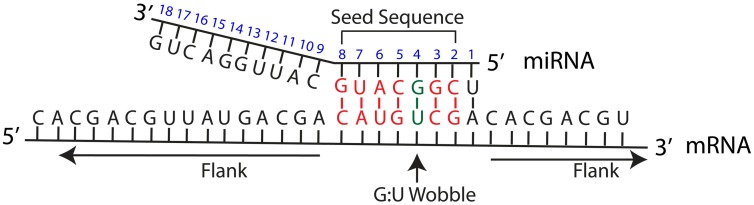
\includegraphics[width=0.7\textwidth]{Figures/seed_match}
	\caption{Example of miRNA targeting.}
	\label{fig:mirna_binding}
\end{figure}

%----------------------------------------------------------------------------------------

\section{MiRNA target prediction}
Before miRNA target prediction tools were available, possible miRNA binding sites were
determined manually. These target sites were later confirmed by laborious and inefficient techniques such as site-directed mutagenesis and other experimental methods. The identification of the first targets for the let-7 and lin-4 miRNAs led to the idea that miRNAs have a pattern in targeting genes which could be used to develop target prediction algorithms \cite{first_predictions}.

Originally gene targeting by miRNAs was believed to be the result of their binding to the 3'UTR of the target mRNA \cite{multiple_binds}, however recent studies \cite{grosswendt} have confirmed gene regulation as a result of the binding of the miRNA to the coding region as well as to the 5'UTR. Furthermore, computational evidence suggests that regulation via the binding of the miRNA to the coding region differs in comparison to the binding pattern seen at the 3'UTR. In particular, it's suggested that miRNAs target the coding regions of mRNAs with short 3'UTRs \cite{functional_sites}.

Another key factor in target prediction is that 3'UTRs are prone to change under different conditions which might result in the elimination of the target site. Binding in the coding region on the other hand may instead present an evolutionary advantage for the cell as it could help in the preservation of the miRNA binding site \cite{mirna_targets}. 

\subsection{Features and methodologies}
While many miRNA targets have been computationally predicted only a limited number
have been experimentally validated. Moreover, although a variety of miRNA target prediction algorithms are implemented, results amongst them are generally inconsistent and correctly identifying functional miRNA targets remains a challenging task.

The average performance of target prediction tools, which typically identify approximately 80\% of known miRNA targets, indicates that the mechanisms associated with miRNA-regulated processes remain poorly understood. Thus, there is a room for novel approaches to improve the knowledge of the rules that govern their targeting process \cite{targeting_rules}

The various methodologies implemented use several different approaches and analyze a wide range of features for this task. Almost all target prediction methods are rule-based or adopt machine learning methodology with varying success. Rule-based systems incorporate various human-crafted descriptors to represent miRNA:gene target binding (e.g. type of pairs in the site, binding stability, or conservation of the target site among species). Machine learning techniques also use those descriptors, but as input features to machine learning models. The limitation of both these approaches is indeed the process of feature selection and representation, which is constrained by
the use of human selected descriptors to model a process that is not fully understood.

The most common characteristics used in miRNA targets identification are \cite{common_features}:
\begin{itemize}
	\item seed region complementarity
	\item free energy
	\item site accessibility
	\item conservation
\end{itemize}

\subsubsection{The seed region}
Targeting patterns are very different between plants and animals. Plants, in fact, show a near perfect complement between their miRNA and the respective target mRNA. On the other hand animal miRNAs bind their targets with only partial complementarity. In particular, a region of about 6 to 8 nucleotides in length at the beginning of the miRNA is of crucial importance in the targeting.  This short subsequence is called \emph{seed region} and it comprises the nucleotides between the second at the eighth (the seed sequence in Figure \ref{fig:mirna_binding}) starting from the 5' end. 
The seed region is very important because it binds to the target mRNA leading to the regulation of the gene in question \cite{mirna_overview}.

Undoubtedly the seed region is one of the most commonly used miRNA traits for target prediction. This seed-centric view, in fact,  has been supported by structural studies \cite{structural_basis} and a widely cited report  \cite{canonical_target} that investigated the importance of other (non-canonical) regions within a miRNA concluding that their contributions had relatively low relevance compared to the (canonical)
seed region. More recent experiments, however, have highlighted a role for the entire miRNA, suggesting that a more flexible methodology is needed \cite{helwak}.

\begin{figure}[hbt!]
	\centering
	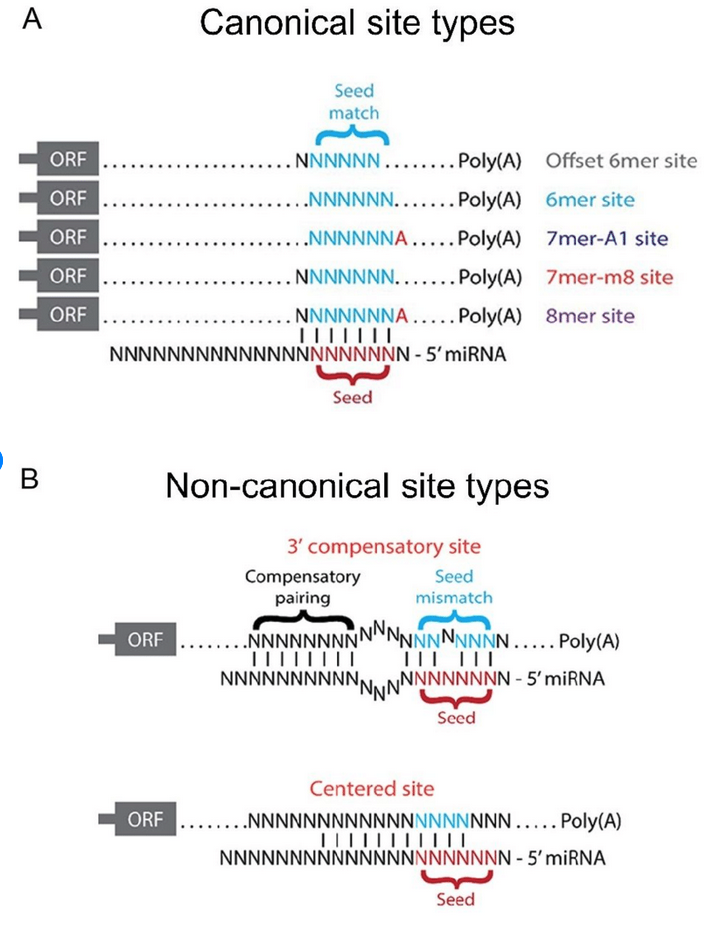
\includegraphics[width=0.5\textwidth]{Figures/canonical_noncanonical}
	\caption{Example of canonical and non-canonical binding sites.}
	\label{fig:canonical_binding}
\end{figure}

\subsubsection{Free energy}
The free energy, also called hybridization energy,  is defined as the energy released by the pairing between the miRNA and mRNA and it can be used as the measure of the stability of the bond. In fact a stable bond is considered more likely to be a functional target of the miRNA. However, since measuring this quantity directly is difficult, usually the change of free energy during a reaction is considered ($\Delta G$). Reactions with a negative $\Delta G$ have less energy available to react in the future, hence they result in systems with an increased stability. By predicting how the miRNA and its candidate target hybridize, regions of high and low free energy can be inferred (Figure \ref{fig:free_energy}) and the overall $\Delta G$ can be used as an indicator of how strongly bound they are \cite{free_energy_survey}. The lower this value the more stable the binding.

\begin{figure}[hbt!]
	\centering
	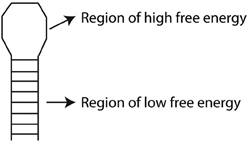
\includegraphics[width=0.5\textwidth]{Figures/free_energy}
	\caption{A hairpin loop is shown with the loop corresponding to a region of high free energy (a positive $\Delta G$) and the stem corresponding to a region of low free energy (a negative $\Delta G$)}
	\label{fig:free_energy}
\end{figure}

\subsubsection{Site accessibility}
Site accessibility is the measure of the ease with which a miRNA can locate and hybridize with its target. After transcription, in fact,  a mRNA assumes a certain secondary structure which can interfere with the miRNA ability to bind to its target site. To understand why this is important, we need to consider that the miRNA:mRNA hybridization involves  a two-step process in which a miRNA firstly binds to a short accessible region of the mRNA and only after, while the secondary structure of the mRNA unfolds, completes the binding.  It is likely that secondary structures contribute to target recognition, because there is an energetic cost to freeing base-pairing interactions within mRNA in order to make the target accessible for miRNA binding. Hence, to assess the likelihood that a mRNA is a target of a given miRNA, the predicted amount of energy required to make the site accessible (the so called site accessibility energy SAE) should be taken into consideration \cite{accessibility_nrg_role}.

The SAE	can be computed as the difference between the free energy cost of opening the mRNA and free energy gained from the intermolecular interaction (Figure \ref{fig:opening_energy}).

\begin{figure}[hbt!]
	\centering
	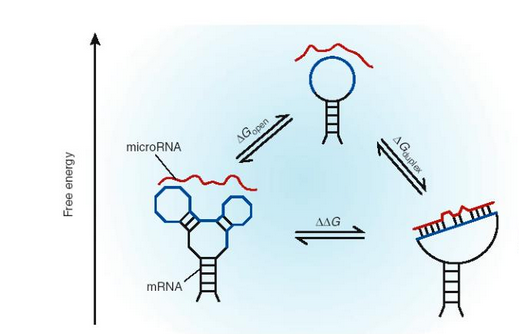
\includegraphics[width=0.7\textwidth]{Figures/opening_energy}
	\caption{Binding of a miRNA to its target mRNA is depicted as a 2-step process. Portion of the mRNA structure must be open before miRNA:mRNA base pairing can be established.}
	\label{fig:opening_energy}
\end{figure}

\subsubsection{Conservation}
Conservation refers to the maintenance of a sequence across species. According to many reports \cite{computational_methods} looking at conserved targets between different species helps reducing the number of false positive results. However, other more recent studies highlighted the fact that this may also increase the number of false negatively identified targets \cite{conserved_pairing}.